% Latex Beamer template following CERN template guidelines (or trying!)

\documentclass[aspectratio=169]{beamer}
\usepackage{xcolor}
\usepackage{graphicx}
\usepackage{multicol}
\usepackage{tikz}

% Code listings with syntax highlighting
%  Require Pygments
\usepackage{minted}

\usetheme{CERN}


% Talk date
% Uncomment this to define a presentation date distinct from \today
\def\mydate{11 Oct 2018}

% Preamble
\title[]{Readout System Enhancements for ATLAS ITk Project }
\subtitle{}
\author[Kyle Beyer , Dylan Hatch]{Kyle Beyer, \texorpdfstring{\url{kyle.beyer@cern.ch} \\ Dylan Hatch ,  \url{dylan.brown.hatch@cern.ch}}{Kyle Beyer , Dylan Hatch}}

% Body
\begin{document}
    
    \cernSplashBlue

    % Title
    {
    \setbeamertemplate{footline}{}
    \setbeamertemplate{navigation symbols}{}
    \frame{\titlepage 
		
      \begin{tikzpicture}[remember picture, overlay]
        \node[anchor=south west, %anchor is bottom left corner of the graphic
              xshift=0.5cm, %shifting around
              yshift=0.5cm]
       at (current page.south west) %left bottom corner of the page
        { 
\includegraphics[width=0.3\paperwidth]{images/mlogo.png} };

        \node[anchor=south east, %anchor is bottom left corner of the graphic
              xshift=-0.5cm, %shifting around
              yshift=0.3cm]
       at (current page.south east) %left bottom corner of the page
        {	
\includegraphics[width=0.23\paperwidth]{images/wlogo.png} };
			\end{tikzpicture}

    }

    \setcounter{framenumber}{0}

    % TOC
%     \frame{
%        \frametitle{Agenda}
%        \begin{multicols}{2}
%            \tableofcontents
%        \end{multicols}
%    }




    
    \frame{
        \frametitle{Acknowledgements}
        We would like to acknowledge the University of Michigan Department of Physics, specifically Jean Krisch and Tom Schwarz, and Steven Goldfarb. 

        We would also like to acknowledge the support of the Lounsbery foundation.   \\
        %More content goes here
      \begin{tikzpicture}[remember picture, overlay]
        \node[anchor=south west, %anchor is bottom left corner of the graphic
              xshift=2.4cm, %shifting around
              yshift=0.4cm]
       at (current page.south west) %left bottom corner of the page
        { 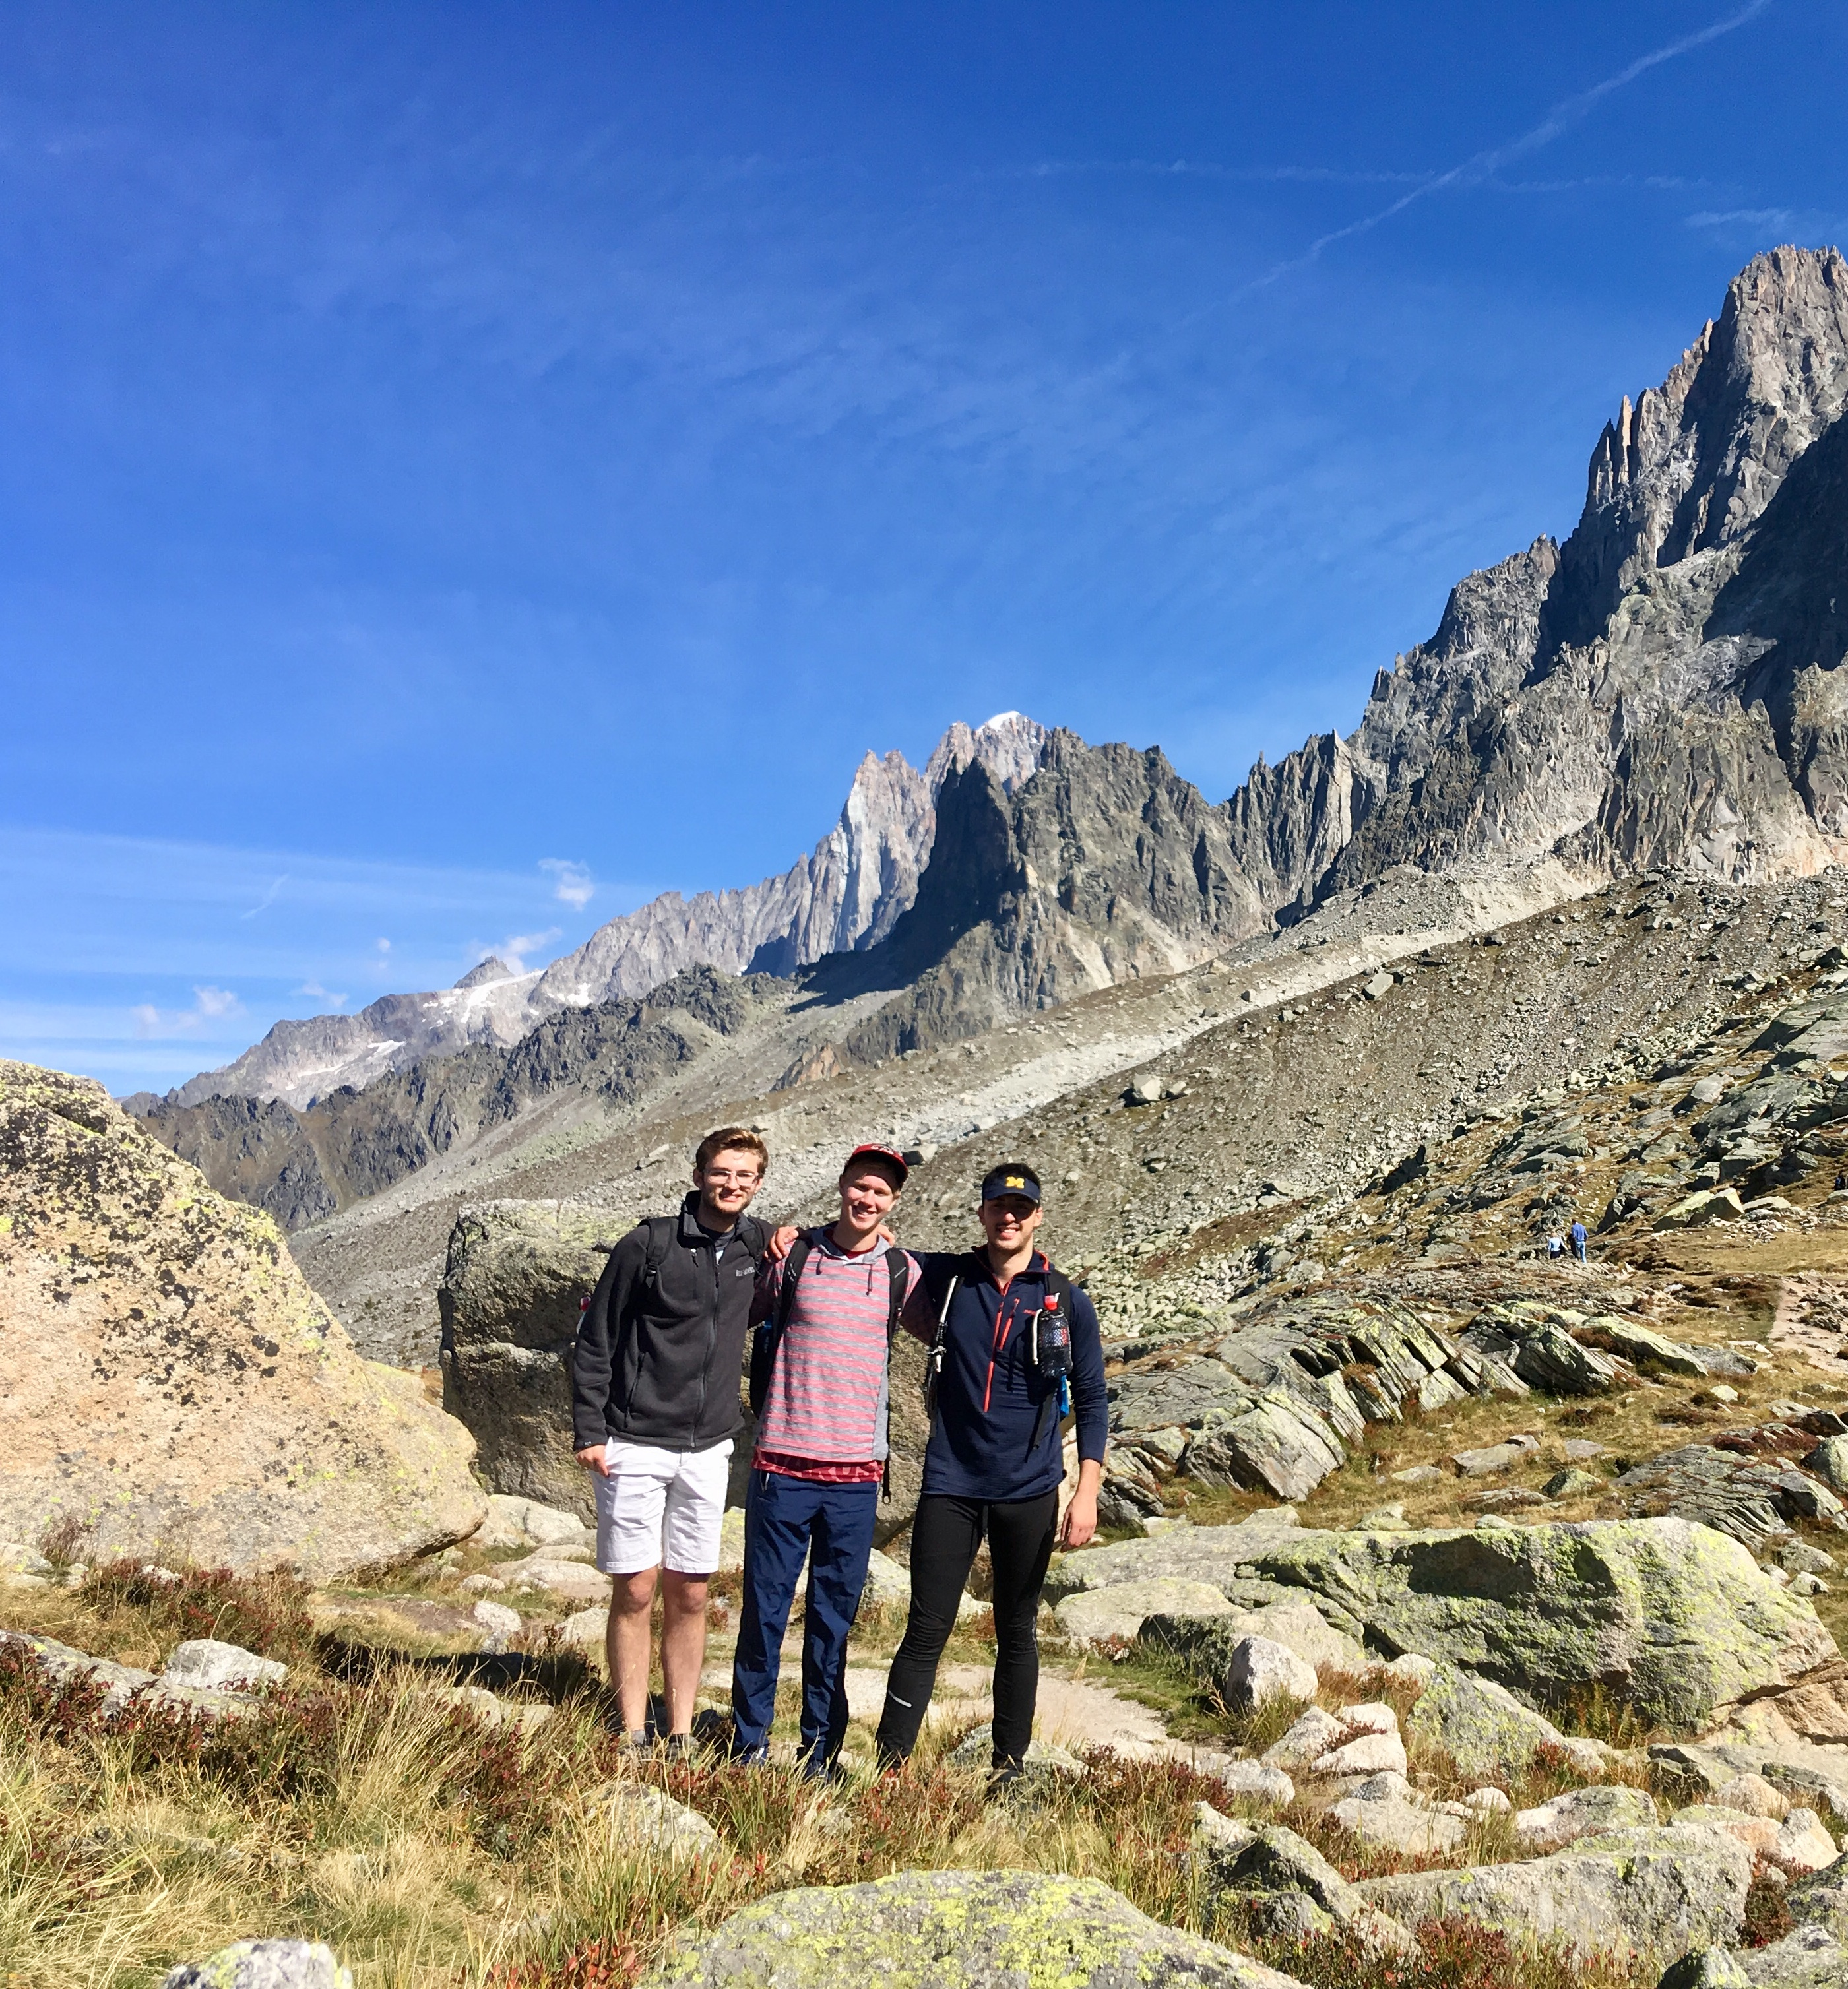
\includegraphics[scale=0.05,trim={0 0 0 35cm },clip]
        {p1-figs/cham.jpg} };

        \node[anchor=south east, %anchor is bottom left corner of the graphic
              xshift=-2.4cm, %shifting around
              yshift=0.4cm]
       at (current page.south east) %left bottom corner of the page
        {	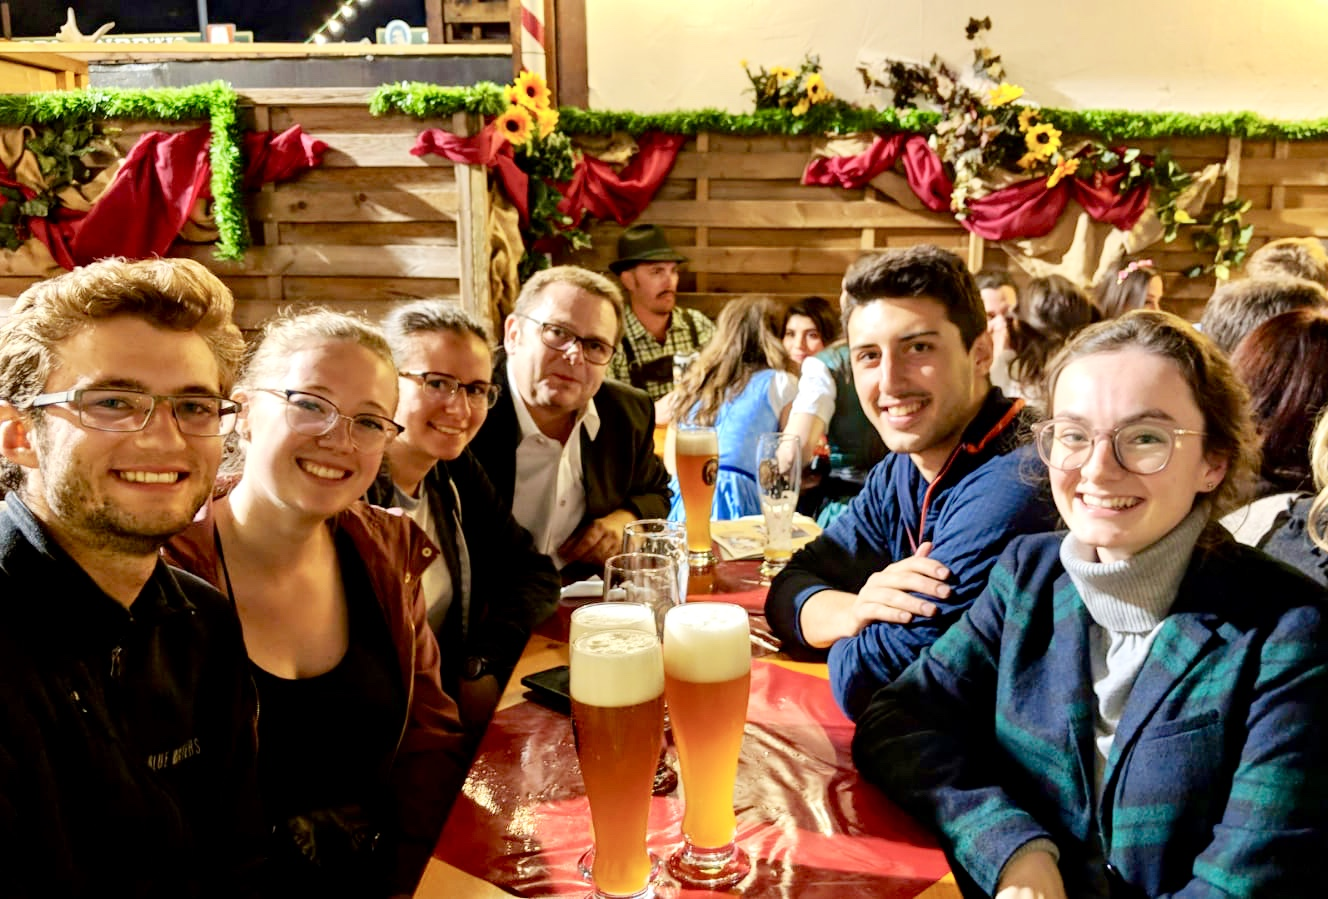
\includegraphics[width=0.33\paperwidth]{p1-figs/okto.jpg} };
			\end{tikzpicture}
        
        
    }

    \section{}
    \cernSplashWhite

\end{document}

